BriefCASE provides access to two analysis tools (GearCASE~\cite{gearcase2020} and DCRYPPS~\cite{dcrypps2019}) that can examine AADL models to detect potential cyber vulnerabilities and suggest requirements for mitigation.
%
Systems engineers are then presented with a requirements management interface (Figure~\ref{fig:req-mgmt}) for viewing the generated requirements and importing them into the model so they can be addressed.  The interface enables engineers to select the requirements they wish to import and assign them unique IDs, or omit them with rationale.  A document of the omitted requirements and rationale is maintained, and may be a required development artifact for some certification domains.  Some requirements can also be formalized as assume-guarantee contracts, enabling formal analysis in AGREE.  Such a requirement will be imported with an associated formal AGREE contract.

\begin{figure}[h]
	\centering
	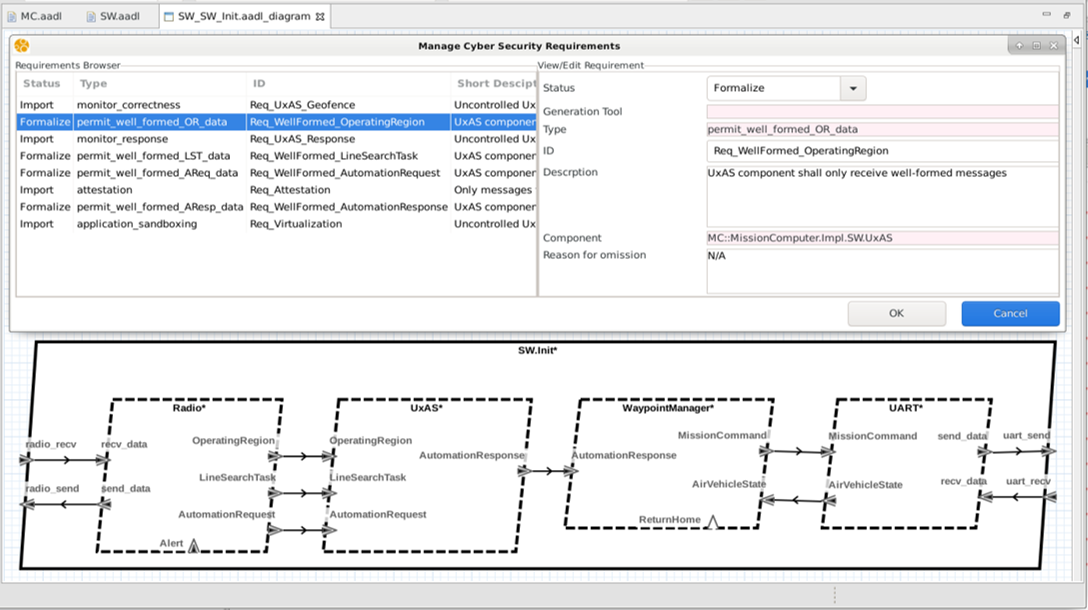
\includegraphics[width=\columnwidth]{figs/req-mgmt.png}
	\caption{Requirements management interface.} 
	\label{fig:req-mgmt} 
\end{figure}

A BriefCASE project contains a repository for requirements.  Imported requirements are represented as Resolute goals to be satisfied.  For example, the well-formedness requirement selected in Figure~\ref{fig:req-mgmt} is imported as the Resolute goal shown in Figure~\ref{fig:req-wellformed-or}.
Initially, the goal is marked \textit{undeveloped}, and does not contain any evidential statements for Resolute to evaluate in order to determine whether the goal has been satisfied.  Running Resolute at this time will therefore produce a failed assurance case. 

\begin{figure}[h]
	\centering
	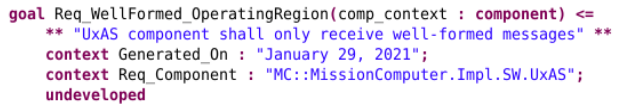
\includegraphics[width=1\columnwidth]{figs/req-wellformed-or.png}
	\caption{Resolute well-formedness requirement.} 
	\label{fig:req-wellformed-or} 
\end{figure}